\documentclass{report}
\usepackage[english]{babel}
\usepackage{microtype}
\usepackage{amsmath,amssymb}
\usepackage{amsthm}
\usepackage[round, authoryear]{natbib}
\usepackage[all]{xy}
\usepackage{graphicx}
\usepackage{framed}
\usepackage{enumerate}
\usepackage{qtree}
\usepackage{mdframed}
\usepackage{tikz-dependency}
\usepackage{float}
\bibliographystyle{plainnat}
\author{}
\title{}

%Define theorem style for definition and metric
\theoremstyle{definition}
\newtheorem{metric}{Metric}
\newtheorem{notion}{Notion}
\theoremstyle{plain}
\newtheorem{definition}{Definition}
\def\citepos#1{\citeauthor{#1}'s (\citeyear{#1})}

%Define new float environment for tables that is boxed
\floatstyle{boxed}
\newfloat{tab}{tbp}{lop}
\floatname{tab}{Table}


\begin{document}
\maketitle
\tableofcontents

\chapter{Introduction}

Ever since ..., many have been inspired by this quote of Warren Weaver, one of the very first researchers to aim for the construction of systems automatically performing translation task.:

\begin{quote}
\textit{When I look at an article in Russian, I say: `This is really written in English, but it has been coded in some strange symbols. I will now proceed to decode.}
\end{quote}

Evidently, automatic translation is not as easily solved as Weaver thought at the time. Over 60 years later, we still have no systems that automatically produce translations with a quality comparable to that of a human translator (anders). The field of Machine Translation has grown much bigger, currently there are (something that indicates the size of the field of Machine Translation), and may different methods have been investigated. This work focuses on one such method: compositional translation.\\
%Explain what compositional translation is (based on compositionality of language, mapping between the grammars generating them. Describe principle of compositionality of translation
In many fields in which translations occur (computer science, logic, philosophy), computational translation is a very common method. The semantics of an expression in a certain logic, for instance, can be unambiguously determined by considering the terms and the methods used to combine them. Translating such an expression into another logical language can be effectively carried out by translating these terms and methods into the terms and methods particular for the second logic. For natural language, compositional translation is not as straight forward.
%words have multiple meanings, sentences are vague and ambiguous, building blocks are unclear blabla
Not only do we have to deal with problems as disambiguation and context, we also do not dispose a set of rules uniquely generating our language. In fact, many have argued against language as a completely compositional system (ref). Examples of arguments against compositionality.\\
I guess a short section about the formal strength of compositionality.


% although not every grammar is suitable for compositional meaning assignment, the class of languages that can be analyzed is not restricted, nor are the meanings that can be assigned: any recursively enumerable language can be generated by a compositional grammar, and any semantics can be dealt with in a compositional way. 
%Is this helpful? Is NL recursively enumerable? What about ambiguity

However, none of this teaches us if compositional translation is a reasonable strategy for translating natural language. Intuitively, it seems reasonable that 'who-did-what-to-whom-relations' are universal for languages, but exploiting this fact in translation has proven to be a non-trivial task. The present work does not aim to develop a model for compositional translation of language, but rather attempts to empirically analyse if it is realistic to aim for one.\\
%Explain how this question becomes practical
Although this question is of theoretical nature, blabla explain that we have to deal with data such that it merely transforms to the question: can we find compositionality in the corpora we are training on, that an be of use in translation models. We will therefore also pay some attention to the use of the results, and make suggestions for future work.

\section*{Related Work}

This is not the first work concerned with the ... phenomena related to compositionality

\cite{fox2002phrasal} investigated if syntactic phrases tend to stay together during translation from French to English.
%Explain how this has to do with compositionality
%Explain how she did this
%Mention issue of phrasal translation
%Discuss her results

Even more directly related to this work is the empirical study presented by \cite{hwa2002evaluating}. \citeauthor{hwa2002evaluating} empirically evaluate the \textit{Direct correspondence assumption (DCA)}, the assumption that for two sentences that are each others translation, the syntactic relations in one sentence directly map to the syntactic relations in the other. %Explain similarity with compositionality of translation principle
%Explain that Hwa argues that the DCA cannot account for some well known and fundamental linguistic facts
%Explain that this is also what they show
%Explain what she does after (making linguistic adaptations)
%Discuss these result: problem with building blocks, still doesn't show that ocmpositional translation isn't possible.. (what else?)


\section*{Thesis Outline}

%Rewrite this when the rest is written
As mentioned before, the primary goal of this thesis is to investigate whether predicate-argument relations are preserved during translation. To do so, a tree will be searched that respects both the alignment (completely) and as much of the predicate-argument relations present in the source sentence as possible. The resulting tree will be scored according to how many of the predicate argument relations were allowed by the alignment, thus yielding a compositionality measure for the sentence.\\
The following chapter will give some theoretical background: it will explain the notion of alignment-respecting trees (anders) and provide some information on the grammar formalism used to extract predicate-argument relations.\\
Chapter give more information on the implementation of the research, while the actual experiments and their results will be presented in chapter 
%We probably also need a section about compositionality (lets see how that is gonna fit in)
%Describe the rest





%%%%%%%%%%%%%%%%%%%%%%%%%%%%%%%%%%%%%%%%%%%%%%%%%%%%%%%%%%%%%%%%%%%%%%%%%%%%%%%%%%%%%%
%%%%%%%%%%%%%%%%%%%%%%%%%%%%%%%%%%%%%%%%%%%%%%%%%%%%%%%%%%%%%%%%%%%%%%%%%%%%%%%%%%%%%%
%BACKGROUND ON MT AND TRANSFER MODELS

\chapter{Transfer Models in Machine Translation}

%%%%%%%%%%%%%%%%%%%%%%%%%%%%%%%%%%%%%%%%%%%%%%%%%%%%%%%%%%%%%%%%%%%%%%%%%%%%%%%%%%%%
%%%%%%%%%%%%%%%%%%%%%%%%%%%%%%%%%%%%%%%%%%%%%%%%%%%%%%%%%%%%%%%%%%%%%%%%%%%%%%%%%%


Machine translation is a very complex problem, to which many approaches have been tried. In this thesis, we focus on one such approach: the transfer method.   After a short introduction to the beginning of Machine Translation (MT), the focus will thus mainly lay on models that use this method. It does not claim to give a complete overview of these. MT is an enormous field in which many models have been developed, most of which are hybrid in the sense that they borrow from different approaches to complete different parts of translation. For more complete overviews of MT and SMT, the reader is referred to \cite{hutchins1992introduction} (MT), \cite{somers1999review} (EBMT) and \cite{koehn2008statistical} (SMT).


\section{Early Transfer Models}
Machine translation was, rising as a field of research almost immediately after the emergence of the first computers, one of the very first problems to be tackled (ander woord) by computers.
%somewhat more general and introductory statements?

The very first approaches to solve the problem, also called the first generation approaches, were more or less direct: sentences were treated as structureless sequences of words that can be directly mapped to words in another language. In such an approach, relations between words or other structural aspects of the sentence are not considered. Clearly, such a strategy is only reasonable if source and target languages are structured almost identical: a translation whose structure deviates from the structure of the original sentence will never be found. Unfortunately for MT researchers, natural languages are not ordered in this fashion, and the direct approach of the first generation models was not very successful, leading to translations that were incomprehensible, not fluent and often not even meaning preserving.

The failure of the first generation models lead to a second generations of models using indirect methods, that laid the groundwork for the models considered in this paper. The main idea of the second generation systems was to use analyse the source sentence into an intermediate representation that was supposed to somehow convey the semantic structure (or `meaning') of the sentence, and map this representation to an intermediate representation in the target language. From this intermediate representation, the translation of the sentence in the target language could be derived. The process of mapping representations in one language to representations in another is called transfer.

An extreme case of the transfer method is the one in which the intermediate representation is a universal one. Such a representation, called interlingua, can be seen as a description of the meaning of the sentence independent of any natural language. The transfer part is therefore reduced to the identity mapping, and translation consists of translating the sentence to an independent meaning representation and deriving the target sentence from this representation. This is attractive from a theoretical point of view, as it addresses the problem on a fundamental level, but is very hard, especially when the meaning space is unrestricted. Some researchers have succeeded in writing rather successful translation models for very small domains (give examples!!), but these days (anders) finding a formal semantics that can capture all of human language is an independent research field, that has grown apart from machine translation (anders).

\begin{figure}[!ht]
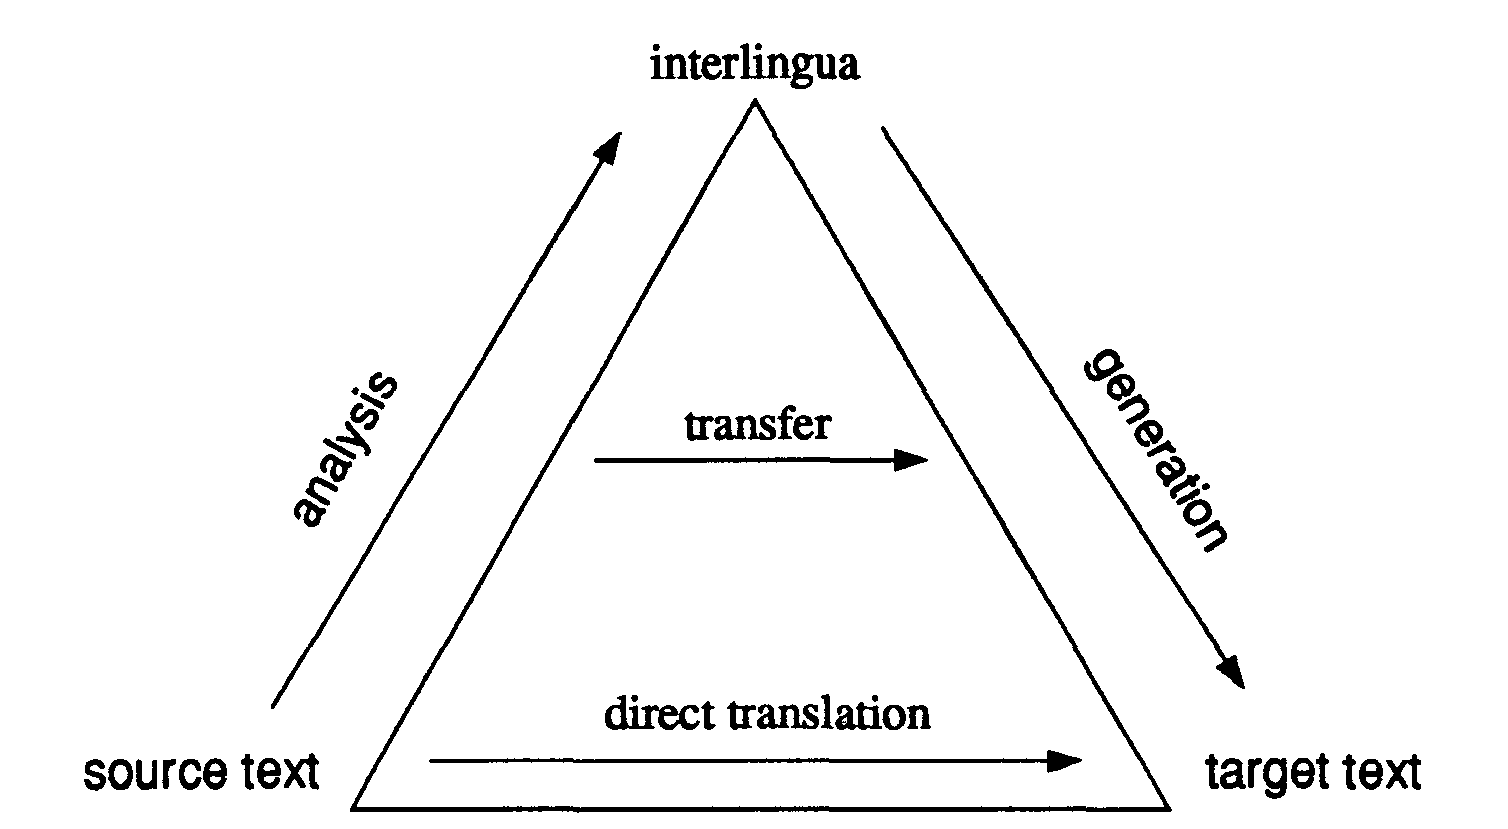
\includegraphics[scale=0.2]{translation_triangle.png}
\caption{Vauquois pyramid?}\label{fig:triangle}
\end{figure}

The three translation methods described can be pictured in a pyramid, showing how they are related (Figure \ref{fig:triangle}). This pyramid also shows that, although direct translation and interlingua are two extremes that are not so flexible, the tranfer method can be employed in different ways varying the distance from source and target text to intermediate representation (analysis and generation, respectively), and with this the distance between the intermediate representations. This point will be discussed more extensively in the next chapter.

\section{Early Statistical Models}

Driven by the thought that language it too rich to formalize, a new line of research came of the ground, that was not primarily based on linguistic knowledge, but on large pairs of text that were translations of each other (parallel corpora). In the beginning, the corpus based systems seemed to be rival to the existing linguistically oriented paradigm, but soon people concluded that the two approaches were not actually conflicting, and nowadays most models combine the two of them.

Corpus based models can be roughly divided into two main categories.\footnote{This distinction is theoretically not cut and clear and in this paper mainly suggested to ...} Models of the first category are directly based on analogy, when translating a sentence, they try to find examples in the corpus similar to (fragments of) the sentence and generate a translation by recombining them. This part of machine translation is often called Exemplar Based Machine Translation. Early EBMT models will not be further discussed (a detailed discussion can be found in \cite{somers1999review}). The early MT researchers had the misfortune that computational standards were not as they are today and their models often only treat small sub languages, are computationally not executable and certainly not scalable. Many of the idea's investigated came back in later papers about MT (e.g. consider \citepos{furuse1992example} hierarchical phrases), although it is unclear if they were inspired by earlier papers or just reinvented.\\
The second category is more interesting to the current work. In models of this category, appositely called statistical machine translation models, parallel corpora are not used to match and recombine, but to statistically decide on the parameters of another model. Even though the first statistical models seemingly took a step back to the direct translation approach again and considered no linguistic information whatsoever, they were (at least result wise) an enormous improvement to any model existing at the time. As these systems were primarily word-based, they do not fall into the category of models discussed in this thesis. However, the models we will discuss are founded on the notions and concepts introduced with these first word-based models, so we will devote a section to them (and their phrase-based extension) nevertheless, before getting back to transfer-models.

\subsection{Statistical Word-based Models}

The first working statistical MT model was presented in 1990, by \cite{brown1990statistical}. This paper was based on earlier work of the same research group \citep{brown1988statistical}, and was further worked out in a later paper \citep{brown1993mathematics} and inspired by Weavers idea \citep{weaver1955translation} to use information theory to reach automatic translation. Their models, now known as `the IBM models' follow the noisy channel approach, modelling the probability $P(t|s)$ that $t$ is the translation of $s$.\footnote{In the literature, this probability is often expressed as $P(e|f)$, as the first IBM models were focussed on translation from French to English. However, this can be quite confusing for the reader, and in this paper we will stick to the more general $t$ for target and $s$ for source.} This probability is then expressed using Bayes' theorem resulting in the following expression (by the authors called The Fundamental Equation of Machine Translation) for the desired translation $\hat{t}$:

\[
\hat{t} = \operatorname*{arg\,max}_t P(t)P(s|t)
\]

The translation task is now split in two: modelling the translation probability $P(s|t)$, and modelling the language probability $P(t)$. The model for $P(t)$, usually an n-gram model, is meant to account for fluency of the target output. Note that the generative model is standard in information theory, the crux of the model resides in how $P(s|t)$ is modelled. In the IBM models, this distribution is modelled by marginalizing over all possible ways in which the words in $t$ could have been generated by the words in $s$, thus $P(s|t) = \sum_a P(s,a|t)$, in which $a$ describes the mapping from target to source words. The 5 IBM models differ in the complexity of the approximation of the conditional probability $P(s,a|t)$, ranging from a very simple distribution in which $a$ is not considered at all (in which case the probability is independent of word-order) to rather complex ones in which $a$ is dependent on several parameters (for details, see \cite{brown1993mathematics}.

%\[
%P(s,a|t) = P(m|t) \prod^{m}_{j=1} P(a_j| a_1^{j-1}, f_1^{j-1},m,t) \times  P(s_j| a_1^{j-1}, f_1^{j-1},m,t)
%\]

All IBM models require a lexical translation probability (i.e. a dictionary like function that specifies the probability of word $w_s$ translating into $w_t$. These probabilities are not directly observable from the parallel corpus (as it is sentence aligned, and not word aligned) and are learned from the data applying the expectation maximization algorithm, that is proved to converge to a global optimum.

\subsection{Statistical Phrase-based Models}

The statistical IBM models led to a huge improvement in translation quality. However, but they still had the same drawbacks as the first generation of direct translation models: no structure or local context was considered and a large amount of natural language phenomena could therefore not be accounted for. A major leap forward was taken with the introduction of (non linguistic) phrases as basic units in translation models (\cite{wang1998grammar,och1999improved}??). In this context, a contiguous sequence of source words is said to be a phrase is it translates into a contiguous sequence of target words, i.e. the words in the source phrase are aligned only with words in the target phrase, and vise versa. \citep{och2004alignment}. Keeping the architecture (more or less) the same, using phrases instead of words allowed to model to use local context during translation. Phrases based translation models can therefore capture (short) contiguous idiomatic translations, as well as small insertions and deletions and local reordering. E.g. both `la casa' and `il casa' are reasonable word-for-word translations of the English phrase `the house'. `il casa' is, however, not a grammatical string in Italian. The latter observation could be easily captured by a phrase-based model, as `the car' could be translated as one unit, but would be much harder to model in a word-based model. Furthermore, a word-based model would never be able to get the correct idiomatic translation of a phrase like 'kick the bucket', while a phrase-based model would have little trouble with that (provided this specific idiomatic phrase was present in the training corpus). (anders) However, such models still suffer from the fact that no structure beyond the phrase level is taken into account.\footnote{Moreover, phrase based translation knows many practical problems, that will not be further discussed here.} Attempts to incorporate syntactic structure by linguistically motivate the selection of phrases \cite{koehn2003statistical,tinsley2009exploiting} turned out unfruitful, and the focus of the MT-world shifted back to more structure-based models.

\section{Statistical Transfer Models}

The shift of the field to more transfer-based models did not happen overnight. Some researchers were exploring statistical rule-based models even before the first phrase-based model was presented. Over the last 15 years, \textit{very} many models exploring structure beyond the phrase-level have been presented, many of which were hybrid models combining several different strategies. 
In this section, the focus lies primarily on models that rather explicitly search for a mapping between source and target language structures. Note that this excludes approaches like \citepos{yamada2001syntax}, in which, even though source side syntax is clearly incorporated, the mapping from source to target syntax is not explicitly modelled. The overview of syntax-based models presented in this section is thus far from complete, and mainly serves to give a gist of what has happened in the rule-based MT-world. For a more general overview, consult for instance \cite{koehn2008statistical}, in which also more attention is paid to decoding, which will not be considered at all in this paper.
%We also do not consider the probability model


An approach that has received much attention is learning a synchronous context free grammar (SCFG) from a parallel corpus.\footnote{In fact, also other types of synchronous grammars were induced from parallel corpora, which we will get back to later (anders)}. Even approaches that are not explicitly concerned with SCFG's, can often be interpreted as such. Formally, a SCFG is defined as a set of rules of the form 

\[
X \to \langle \gamma , \alpha , \sim \rangle
\]

In which $\gamma$ and $\alpha$ are sequences of terminals and non terminals in the source and target language, respectively, and $\sim$ is a one-to-one correspondence between the terminals and non terminals in $\gamma$ and those in $\alpha$ (anders). SCFG's implicitly model reordering phenomena and non-contiguous phrases. 

One class of syntax-based models is trained by parsing both source and target sentences with a linguistic parser and finding a mapping between them. The model would then take a linguistic parse tree of the source sentence as input, and output this to a target side structure. This approach is taken by, among others, \cite{lin2004path}, \cite{galley2004s} and \cite{poutsma2000data}. 
\citeauthor{lin2004path}\\ %discuss lin
\citeauthor{galley2004s}\\ %discuss galley
\citeauthor{poutsma2000data}\\ %discuss poutsma
\cite{groves2004robust}??

\citeauthor{wu1997stochastic} points out, that the `parse-match-parse'-method used by such purely linguistically informed transfer methods, is susceptible to some weaknesses. First of all, appropriate and robust monolingual grammars (and parsers) may not be available. Current monolingual parsers for English are of very high quality, as well as parsers for some other western languages and Chinese (??), but for the lion's share of languages high quality parsers do not exist. Secondly, monolingual grammars are not designed for translation purposes, and grammars of two different languages are therefore not necessarily as compatible as possible.\footnote{A more detailed discussion of this issue can be found in \cite{rosetta1994compositional}. This issue will be further discussed in the next chapter??}.
%Maybe discuss chiang here?
\citeauthor{wu1997stochastic} presents a model that attacks these weaknesses, and is at the heart of many later approaches: the inversion transduction grammar (ITG). The general ITG framework can be formulate as a synchronous context free grammar, and thus does not differ from aforementioned linguistic approaches in this aspect. However, in the ITG framework as presented by \citeauthor{wu1997stochastic} not only the rule correspondences are learned from the corpus, but also the rules themselves. The non-terminal labels are thus not necessarily linguistic constituency labels, but are motivated by the translation data. Learning such grammar rules is associated with computational issues: longer rules can represent a larger set of reordering phenomena (\cite{simaan2013hats}), but also require more computational power. Even without considering any non-terminal labels, the number of rules that can be extracted from a sentence pair without any restrictions grows exponentially with the length of the sentence (GIVE SOMEWHAT MORE EXACT COMPUTATIONS OF THIS NR), and can thus not be all included in a grammar. Restricting the set of structures such that the resulting set shows how the sentence is recursively built up, has been a great challenge for MT (anders). 
%Explain how Wu did this himself
This section will proceed with discussing the different ways that have been proposed to do so.
An interesting and elegant approach is the one taken by \cite{chiang2005hierarchical}. Instead of directly inducing an SCFG, he proposes a new kind of phrases that consist of both words and sub phrases: hierarchical phrases, that act both as discontinuous phrase pair and as a phrase-reordering rule. Formally, the hierarchical phrases can be seen as productions of an SCFG.
%Gluerules
 The number of such translation rules in a 1-1 monotone sentence pair is $\mathcal{O}(n^6)$ \citep{quirk2005dependency}, \cite{chiang2005hierarchical} filters his grammar by excluding rules that %Explain how Chiang exludes rules
\cite{chiang2005hierarchical} were the first to present a rule based system that outperformed a state-of-the-art phrase-based system.
There are two important things to notice about \citepos{chiang2005hierarchical} hierarchical phrases\begin{enumerate}
\item By incorporating non-terminals in phrases, \citeauthor{chiang2005hierarchical} presents a rule-based system that still profits from the attractive properties of phrases.
\item The rewrite rules are extracted based on \textit{word alignments}.
\end{enumerate}

%Somehow get the link to factorizing alignments



% to maximize the chances of covering arbitrary new data, the units should be as small as possible 


Explain who has tried this after Wu (\cite{eisner2003learning},\cite{blunsom2008bayesian})
Get to --> decomposing word alignments (\cite{zhang2008extracting}



\begin{enumerate}
\item \cite{quirk2005dependency,quirk2006dependency} I think this one is quite important
\item \cite{eisner2003learning}
\item \cite{zollmann2006syntax}
\item \cite{melamed2004generalized}
\end{enumerate}



%%%%%%%%%%%%%%%%%%%%%%%%%%%%%%%%%%%%%%%%%%%%%%%%%%%%%%%%%%%%%%%%%%%%%%%%%%%%%%%
%%%%%%%%%%%%%%%%%%%%%%%%%%%%%%%%%%%%%%%%%%%%%%%%%%%%%%%%%%%%%%%%%%%%%%%%%%%%%%%

\chapter{The theoretical backbone of transfer models}

%%%%%%%%%%%%%%%%%%%%%%%%%%%%%%%%%%%%%%%%%%%%%%%%%%%%%%%%%%%%%%%%%%%%%%%%%%%%%%%
%%%%%%%%%%%%%%%%%%%%%%%%%%%%%%%%%%%%%%%%%%%%%%%%%%%%%%%%%%%%%%%%%%%%%%%%%%%%%%%

%SCFG's assume isomorphic structures

As seen in the previous chapter, syntax-based models attempt to find structural representations of sentences in different languages and a function that maps the representations of sentences in one language to the representations of sentences in another if and only if the sentences are each others translation. The types of grammars (the objects generating the representations) and the mappings between them differ from model to model. What these models have all in common, is that they assume that such grammars and mappings exist. In this chapter, we will explain and analyse what the implications of these assumptions are for natural language. (anders) We claim that these assumptions are in fact equivalent to the well-known principle of compositionality of translation:

\begin{quote}
Two expressions are each others translation if they are built up from parts which are each other's translation, by means of translation-equivalent rules (ref??)
\end{quote}

Evidently, if translation between any two languages obeys this principle, representational systems and mappings between them can be found. Conversely if two (tree) representation and a function between them can be found, this function can be seen as a translation-equivalent rule and its input and output as parts and their translation.

The principle of compositionality of translation holds some thoughts on how translation ought to be. We will discuss these thoughts in the following sections.

%What are the assumptions that are implicit in this principle?
% -translation is literal
% -language is compositional
% -languages have a similar semantical structure

\section{Compositionality of Language}

On of the assumptions constituting the principle of compositionality of translation is that languages can be described by means of a compositional grammar, i.e. they are compositional themselves. Compositionality is a property possessed by most artificial languages. The meaning of an expression in a logical language, for instance, can be unambiguously determined by considering the atoms and the rules used to combine them. For programming languages, a similar statement can be made. The following principle, analogous to the principle of compositionality of translation and known as `the compositionality principle' describes this property:

\begin{quote}
Meaning of an expression is a function of the meaning of its parts and syntactic rule by which they are combined \cite{partee1984compositionality}
\end{quote}

To what extend natural languages can said to be compositional is an issue that has yet to be sorted out. Although the compositionality of some part of natural language is undeniable - we can understand sentences we have never heard before because we know the words in it and we are familiar with the methods that can be used to combine them - many have argued against compositionality of natural language as a whole. An often heard counter argument is the existence of idiomatic expressions, whose meaning can clearly not be derived from the meaning of its parts, and scope and reference ambiguities.\footnote{I undoubtedly do the arguments against compositionality short (??), but a detailed discussion of compositionality is outside the scope of this paper... (anders)} As for the latter, it is hard to even make a statement about this with the principle as given above, that is highly underspecified. The power of a compositional grammar depends a great deal on the notion of parts meanings and rules in this grammar. That is to say, in theory it is possible to include all idiomatic expressions along the words as basic units in the grammar (in some cases this might result in a grammar that intuitively does not at all seem compositional any more). 

%This section should be rewritten
There are a couple reasons why an elaborate discussion of the compositionality debate is outside the scope of this paper. Firstly, the main contribution of this paper is an empirical analysis of the level of compositionality that can be found in translation data. Although this question has a theoretical background, as we are are working with real life data, the answer will have a practical nature, and will hopefully show if languages contain \textit{enough} compositionality to be useful in translation. Secondly, arguments against compositionality are often focussed on ambiguous sentences that cannot be assigned distinct syntactic structures. However, disambiguation is a separate issue in MT, that this paper is not concerned with. Moreover, note that these kinds of ambiguity causing non-compositional meaning derivations do not necessarily have to be a problem for translation. Consider for instance the sentence `Two men carry two chairs'. Although this type of ambiguity is troublesome for a compositional analysis \citep{pelletier1994principle}, it does not impair the possibility of compositionally translating to Dutch, as the Dutch sentence `Twee mannen dragen twee stoelen' is ambiguous in the exact same way. (dit is echt een draak van een zin)



An detailed discussion of compositionality by one of the advocates of compositionality can be found in \cite{janssen1996compositionality}. 


%arguments often focus on rare exceptions and contextual ambiguities. function doesn't have to be bijective
%Explain that current work doesn't focus on resolving ambiguities, and also that such things are maybe different for translation?
% Take something from the \cite{janssen1996compositionality} article to explain that compositionality is quite strong, depending on the grammar and the building blocks --> idiomatic expressions

In this paper, \citeauthor{janssen1996compositionality} also shows that although not every grammar is suitable for compositional meaning assignment, the class of languages that can be analysed is not restricted, nor are the meanings that can be assigned: any recursively enumerable language can be generated by a compositional grammar, and any semantics can be dealt with in a compositional way. \textit{Finding} algebra's that describe the meaning and syntax of a language is of course not a trivial task.

\section{Translation is Literal}

Apart from assumptions about the languages involved, the principle of compositionality of translation also makes assumptions about the translation process itself. First of all, it assumes that translation should not only preserve meaning, but also form (as much as possible). In other words, it assumes that translation is literal. Generally, this is helpful when deciding about the adequacy of a translation. An example that illustrates this is the following: \textit{all ravens are black} is an adequate translation of the Dutch \textit{alle raven zijn zwart}, but the logical equivalent sentence \textit{if something is not black it is not a raven} is not \citep{landsbergen1989power}.  However, even without regarding idiomatic translations, that will be considered later, a translator can have many reasons to prefer a more free translation, even if a literal alternative is present. Although this is a real issue in practice, machine translation is by far not developed enough to be concerned with style issues and throughout this paper will be assumed that translation is as literal as possible.

\section{Translation is Compositional}

After having discussed two important assumption that underpin the principle of compositionality of translation, we get to the main point of the principle (ander): translation is compositional, i.e. there exist a systematic mapping between the compositional grammars of two languages.
GIve some examples of seemingly non-compositional phenomena that can still be treated compositionally (\cite{landsbergen1989power}, \cite{rosetta1994compositional})

%Say something about that the grammars need to be tuned to each other, for instance, the need to have the same basic units.

%Maybe say something about the algebraic definition too?

%Consider the Rosetta book again.

%for more examples, refer to landsbergen

%Landsbergen also gives an example for which no compositional solution is found (cross the river swimming), explain that this is a theoretical problem rather than a practical one. Solution is not elegant, but a grammar automatically derived from a parallel corpus won't be elegant anyways :p


%Maybe extra section on minimallity? 

%%%%%%%%%%%%%%%%%%%%%%%%%%%%%%%%%%%%%%%%%%%%%%%%%%%%%%%%%%%%%%%%%%%%%%%%%%%%%%%%%%%%
%%%%%%%%%%%%%%%%%%%%%%%%%%%%%%%%%%%%%%%%%%%%%%%%%%%%%%%%%%%%%%%%%%%%%%%%%%%%%%%%%

\chapter{An Empirical Study}

%%%%%%%%%%%%%%%%%%%%%%%%%%%%%%%%%%%%%%%%%%%%%%%%%%%%%%%%%%%%%%%%%%%%%%%%%%%%%%%%%%%%
%%%%%%%%%%%%%%%%%%%%%%%%%%%%%%%%%%%%%%%%%%%%%%%%%%%%%%%%%%%%%%%%%%%%%%%%%%%%%%%%%

In articles about syntax-based translation models the assumptions discussed in the previous chapter are are rarely mentioned, let alone questioned. Moreover, the evaluation of the models presented is based on the performance of an implemented version of them that is often, due to computational reasons, not even completely equivalent to the version presented. Furthermore, the hybrid nature of models makes the evaluation of the transfer part even fuzzier, as it is not clear which parts of the model are responsible for the results. The current work deviates from this research, in presenting an exploration of the underlying assumptions. Such an analysis is of theoretical importance, but can also serve as an estimate of how far syntax-based translation models can actually bring us and possibly even give information on how to proceed.

The current chapter describes the experiments conducted for this paper (anders). The outline of the chapter is as follows: we will first discuss a number of empirical studies on the recursive properties of translation data. Some of them are pure analyses, while others are mainly focussed on improving performance of a specific model or method, but report some empirical results during the process. After the related work, we will continue with a description of a new experiment (blabla)


\section{Related Work}

%Reread + check of references in paper khalil nog iets opleveren
%consider \cite{huang2009binarization}
%\cite{gildea2006factoring} for arguments for minimal rules

Most empirical studies focus on the explanatory power of transforming linguistic parse trees. Even though they are ran on different datasets (and different language pairs) and use different criteria, they all find that permuting children in a linguistic constituency trees is not powerful enough to account for the reordering phenomena present in translation data, manual or automatic.

An often cited study is the one carried out in \cite{fox2002phrasal}. \citeauthor{fox2002phrasal} investigates the degree of phrasal cohesion across English and French. She counts the number of times the alignment spans of constituents overlap or `cross'. She uses the corpus created by \cite{och2000improved}, containing 500 manually aligned sentences from the Canadian Hansard corpus. The alignments are of type S (on which all annotators agreed) and P (in which annotators disagreed or were uncertain). Although she distinguishes different conditions, we will only report on her results including all alignment links. She concludes that crossings - even after phrasal translations, that necessarily result in crossings, are filtered out - are too prevalent to ignore (on average 2.854 per sentence). Furthermore, she observes that dependency parses have better cohesive properties than constituency parses (2.714 per sentence). \footnote{With a manual analysis of the crossings in the constituency parses she shows that many of them are not due to the lack of phrasal cohesion, but are often caused by errors in syntactic analysis or rewording and reordering in the translation. Her analysis, however, included only the crossings of the S alignments, that constituted only a small part of the total set of crossings.}

Regarding constituency parses, a similar conclusion was drawn in \cite{galley2004s}. \citeauthor{galley2004s}, who analized the same corpus as Fox, concentrated on finding transformation rules based on larger fragments of trees. He plotted the coverage of the grammar against the maximum depth of the rules in the grammar. For the manual aligned Hansard corpus, he found that one depth rules (that are equivalent with child-reordering) could only explain 19.4\% of the corpus.

A third study worth mentioning is the study presented in \cite{hwa2002evaluating}, in which the Direct Correspondence Analysis is evaulated. \citeauthor{hwa2002evaluating} evaluated the quality of Chinese dependency parses that were projected directly from English to Chinese, according to a manual alignment. The resulting parses had a very low F-score (38.1), which is not surprising, as every multiple-aligned word and every unaligned target-word will result in an error. \citeauthor{hwa2002evaluating} make a similar observation, but do not aim for a scalable solution: with a small set of linguistically motivated rules they manage to boost the score significantly (to 68.3), but this result is not generalisable and thus hard to learn from. (anders)

Another paper that confirms the inadequacy of child reordering is \cite{khalilov2012statistical}, in which work is presented that focusses on source reordering preliminary to translation. Using LRscore \citep{birch2010lrscore} as a measure of success, they conclude that child-reordering in a constituency tree cannot be used to reach the perfect permutation of source-words in English-Dutch and English-Spanish translation data, even when it is allowed to delete up to 5 layers of nodes in the parse tree. (their results for English-Spanish, however, are surprisingly high: around 94). 

\citeauthor{wellington2006empirical} shows, that if the alignment trees are not restricted to parse trees, the failure rate is much lower. On several datasets (Chinese, Romanian, Hindi, Spanish and French to English), he found that maximally 5\% of the alignments could not be explained by a completely binary tree, while the failure rate for binary trees that were constrained by monolingual parse trees on the English side climbed to 15\% for French/English to 61\% for Chinese/English. Their failure rate for non constrained binary trees is much lower than the one found by \cite{simaan2013hats}, who reported a coverage of 71.46\% of the manual alignments of the Hansard corpus for trees with a maximal branching factor of 2. The coverage of binary trees for automatic alignments was even lower: 52.84\%. This difference between the results of \cite{wellington2006empirical} and \cite{simaan2013hats} is most likely due to a different treatment in alignment links: the latter author used all alignment links in the dataset, while the former treated many-to-one alignment links disjunctively, focussing on lower bounds. \cite{simaan2013hats} also report the coverage of non binarisable permutation trees (andere term, deze nog niet geintroduceerd), which is surprisingly enough not much higher: 72.14\% and 56.56\% for manual and automatic alignments, respectively.


\section{Original Work}

Following \cite{simaan2013hats} and \cite{wellington2006empirical}, we will study the recursive properties of translation data, disregarding conventional syntax at first. We will consider the set of structures defined by the alignment, as defined by \cite{simaan2013hats}. Before explaining exactly how, we will firstly define this set of structures. Although the notation of some of the definitions are slightly adapted to the convenience of this paper, the information presented in the following subsection can be considered summarising parts \citepos{simaan2013hats}.

\subsection{Hierarchical Alignment Trees}

As the name suggests, a HAT is tree defined over an alignment. Although we have no doubt that any reader of this paper is familiar with this concept, for the sake of the completeness we will briefly exemplify.

\subsubsection{Word Alignments} A word-alignment of a sentence pair is a mapping from source to target-words. An arrow from source word $w_s$ maps to target word $w_t$ implies that $w_t$ was involved in the translation of $w_s$ (an example of an alignment can be found in \ref{fig:alignment}). The precise definition of a word-alignment varies from paper to paper, throughout this thesis we will use the following definition:

\begin{definition}
Given a source sentence $s = s_0 \ldots s_n$ and its translation $t = t_0 \ldots t_m$, an alignment $a = \subset \{0,1,\ldots,n\} \times \{0,1,\ldots,m\}$ such that $(x,y)\in a$ iff $s_x$ is translated into $s_y$.
\end{definition}

Note that the absence of a $y$ such that $(x,y)\in a$ means that $x$ is unaligned. In some definitions unaligned words are explicitly included in the alignment by adding an extra $NULL$ token to both source and target sets, and including $(x,NULL)$ (or $(NULL, y)$) in $a$ whenever $x$ (or $y$) is unaligned. 

\begin{figure}
\centering
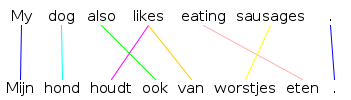
\includegraphics[scale=0.6]{alignment.png}
\caption{A one-to-many alignment of the English sentence `My dog also likes eating sausages.' and its translation `Mijn hond houdt ook van worstjes eten'.%schrijf welke tool is gebruikt
}\label{fig:alignment}
\end{figure}

Alignments can be of several types, which will be of importance for the complexity of our algorithms. A summary can be found in table \ref{table:alignments}.


\begin{table}[!ht]
%Put a box around this thing!!
\begin{tabular}{ll}
one-to-one & $\forall x\forall y \big( (x,y)\in y \to \forall z \big( (z,y)\in a \to z\!=\!x \land (x,z) \in a \to z\!=\!y \big ) \big ) $\\
&\\
one-to many & $\forall x\forall y \big( (x,y)\in y \to \forall z \big( (z,y)\in a \to z\!=\!x \big) \big) $\\
&\\
many-to-one & $\forall x\forall y \big( (x,y)\in y \to \forall z \big( (x,z) \in a \to z\!=\!y \big) \big ) $\\
&\\
many-to-many & - \\
&\\
monotone & $\forall w \forall x\forall y \forall z \big ( \left ( (x,y)\in a \land (w,z)\in a \land x < w \right ) \to y < z \big )$\\
\end{tabular}
\caption{Alignment types, restrictions}
\label{table:alignments}
\end{table}

To make matters easier, we will introduce a change in notation, in which alignments are represented as a special sort permutation, in which numbers of the original sequence are allowed to appear more than once, or not at all. We will call this new representation a set-permutation. A set-permutation is defined as follows:

\begin{definition}
Given a source sentence $s = s_0 \ldots s_n$, its translation $t = t_0 \ldots t_m$, and an alignment $a$, let $a(i) = \{j | (i,j)\in a\}$ be the set with target positions that is linked to source position $i$. The set-permutation $\pi$ uniquely describing $a$ is now defined as the ordered sequence of sets
$\langle a(0), \ldots, a(n) \rangle$
\end{definition}

The set-permutation $\pi = \pi_0, ..., \pi_n$ describing the alignment showed in Figure \ref{fig:alignment} would thus be $\langle {0}, {1}, {3}, {2,4}, {6}, {5}, {7}$. In the following definitions we assume that $\bigcup_{i=0}^n \pi_i$ constitutes a contiguous sequence of numbers. Thus, whenever the target sentence contains an unaligned word, the position numbers of all words after shift one position to the left. (anders) 

\subsubsection{Translation Units} To define a tree over an alignment, we need to have a notion of allowed sub sequences. For this, we use a definition analogous to the definitions of phrase pair used in the first phrase based models \citep{och2004alignment}. A phrase pair is a pair of source and target spans [i,j] and [x,y], respectively, such that at least one word in [i,j] is aligned to at least one word in [x,y], and no words in [i,j] are aligned to words outside [x,y] and vice versa. The phrases consistent with the alignment are thus phrases whose translation is also a phrase. Translated in terms of a set-permutations $\pi$, we get the following definition for a translation unit:

\begin{definition}
A span [$i,j$] representing contiguous sequence $s_i\ldots s_j$ of a source sentence whose alignment is represented by set-permutation $\pi = \langle\pi_0 ,\ldots ,\pi_n$ is a possible translation unit iff the union $(\pi_i\cup \ldots \cup \pi_j)$ constitutes a contiguous range of integers, and for every integer $x \in (\pi_i\cup \ldots \cup\pi_j)$ holds that  $x \notin (\pi_0\cup \ldots \cup \pi_{j-1} \cup \ldots\cup\pi_{i+1}\cup\ldots\cup \pi_n)$.
\end{definition}

The set of translation units consistent with the alignment in Figure \ref{fig:alignment} is thus: {[0,0], [1,1], [2,3], [4,4], [5,5], [0,1], [2,3], [4,5], [1,3], [0,4], [2,5], [0,5]}. In which [x,y] includes all words from position $x$ to position $y$. Note that the word 'like' is not a translation unit on its own, as it translates into two non-adjacent words in the Dutch target sentence. The number of translation units in an alignment depends on the type of the alignment and is largest in case of a monotone alignment, that does not restrict the set of possible phrases at all. A completely monotone alignment of a sentence of $n$ words has $\frac{n\times n+1}{2}$ phrases. Note that unaligned words can cause exponential growth in the number of phrases.

\subsubsection{Alignment Trees} Given the set of translation units, we can define the set of structures according to which the sentence could have been compositionally translated. 

\begin{definition}
%Dit moet misschien nog even anders
Given a source sentence $s = s_0 \ldots s_n$ and the set of its translation units $u = \{u_1,\ldots,u_m\}$. An alignment tree $T$ is any tree satisfying the following conditions 4 conditions:\begin{enumerate}
\item $[0,n]$ is the root of the tree
\item For the set of all nodes $N$ in $T$ holds: $N\supset \{[i,i]| 0\leq i\leq n\}$
\item Every node $n\in N$ is in $u\cap \{[i,i]| 0\leq i\leq n\} $
\item For every node $n\in N$ with children $C_n$ holds $\bigcup C_n$ constitutes a contiguous range of integers.
\end{enumerate}
\end{definition}

An alignment may have many different possible alignment trees. The number of alignment trees can be exponential in the length of the sentence, if no restriction is placed on the branching factor of the nodes. Every alignment can be assigned at least one structure, that is completely flat. A possible alignment tree for the running example alignment can be found in Figure \ref{fig:alignment_tree} (the words of the sentence are included for clarity reasons).

\begin{figure}[!ht]
\Tree [.[0,6] [.[0,1] [.[0,0] my ] [.[1,1] dog ] ] [.[2,6] [.[2,4] [.[2,2] also ] [.[3,3] likes ] [.[4,4] eating ] ] [.[5,6] [.[5,5] eating ] [.[6,6] sausage ] ] ] ] ]
\caption{A possible alignment tree for the alignment of Figure \ref{fig:alignment} \label{fig:alignment_tree}}
\end{figure}

\subsubsection{Hierarchical Alignment Trees}
Explain that they are minimal blabla, which we want because of generalisation properties (chiang ref?) (citaat wellington --> beter in generaliseren)
Say that in the original paper the nodes are decorated with ITG like operations that describe how a target-side tree can be obtained.


\subsubsection{The power of HATs}

Maybe give some examples? Tell what kind of mapping it describes
 write how HATs can account for phenomena as ne ... pas?


\subsection{HAT Selection}



% So I guess I should think exactly what I want to do.
% Firstly, note that HATs receive a rather low score, then show that considering all trees actually yields a rather high score (with manual alignments), this is an upperbound to what can be reached
% thus considering other labels might be fruitful
% Investigation of which labels are generally preserved in the HATs (I think I will write a small bash-script to do this given a list of labels and their counts and a file with parse trees)
% See what conclusions we can draw from this
% Define all CCG like labels and check their consistency with the alignments (i.e. upperbound, all trees)
% parse with all labels or selected labels (HATs)
% Once again output preservance




\chapter{Implementation}



Explain that the main framework scores an alignment according to a given set of preferred relations between nodes that are siblings in the tree, or nodes that are mother and child. Explain that it is designed to be easily extendible for testing different properties of the tree.

Explain that tests were conducted with different evaluation metrics, information about which can be found in the description of the experiments.

%Do not know what level of detail is required here...
Briefly discuss how: for each alignment a grammar is created that uniquely generates all Recursive Alignment Trees. The different productions of this grammar are assigned a score proportional to the preferred number of mother child relations that it generates. (similar to a probability, but not the same). A parser is used to find the optimal alignment tree (i.e. the alignment tree with the highest number of preferred mother child relations), and its score.
%Maybe say something about the scoring and how different things can be tested but that one needs to think about scores for the productions


\section{Implementation}

Open source implementation that consists of different parts

\begin{itemize}
\item the part that deals with the dependency relations, extracts different relations from them and assigns labels to spans
\item part that generates the context free grammars, details about this is implemented? graph approach, spans found by an algorithm similar to Zhangs.. def of phrases is slightly different, an emtpy node can also be a phrase.
\item parser, external viterbi parser from nltk toolkit \citep{bird2009natural}, slightly adapted such that it can dael with scores that are not probabilities 
\end{itemize}

The only thing that is thus required is an evaluation metric

%Show that graph algorithm is sound and complete

%Explain what I did (and will do!)



\section{Dependency Grammar}

%Introduction: maybe some history about dependency grammars and how they came about (refer to phrase structure grammars)

%Explain why dependency relations seems suitable for the task at hand: we want to see if predicate argument relations stay intact, dependencies are predicate argument relations
%Maybe also some arguments from other studies that support the suitability of dependency grammars (higher cohesion dependency grammars fox e.g, work quirk & menezes.

%Describe stanford dependency representation

The Stanford Dependency representation distinguishes five different styles. As an elaborate description of these styles, as well as an extensive list of the relations in all of them, can be found in the Stanford typed dependency manual \citep{de2008stanford}, in this thesis just a short summary will be given.
\paragraph{Basic Dependencies} The basic dependency style contains, as the name suggests, all the basic dependencies present in the sentence. A basic dependency structure is a fully connected projective dependency structure, that is, there are no crossing dependencies.
\paragraph{Collapsed dependencies} In the collapsed representation several dependencies involving function words are collapsed to get direct dependencies between content words. Furthermore, additional dependencies that break the tree structure are considered, which means the resulting dependency graph is not guaranteed to be acyclic or even a tree. There exist another 2 variants of the collapsed dependency representation, one in which conjunct dependencies are propagated, and one in which the dependencies that do not preserve the tree structure are omitted.
\paragraph{Non-collapsed dependencies} The last representation gives the basic dependencies as well as the extra ones which break the tree structure.

%Describe available parsers.
Zeg iets over de beschikbare parsers \cite{de2006generating}
%Probeer misschien nog wat andere literatuur te vinden over dependency grammar

\section{The Best Tree}

Describe that we need a way to decide how good a tree is and that there are different ways to do that. Present evaluation metrics.

\subsection{Shared Notation}

Firstly, we will present some notation that is shared along the different metrics.

\begin{notion}
$T_d$ will refer to a dependency tree of a sentence $s = w_1 \dots w_n$, formed by a set of dependencies $D = \{ (i,j) |$ there is a dependency arrow from word $w_i$ to word $w_j \}$.
\end{notion}

\begin{notion}
If $T_d$ is a dependency tree for $s$, $w$ is a word in $s$ and $i$ and $j$ are the maximum and minimum positions, respectively, that can be reached from $w$ by following the directed dependency arrows. Then span($w$) = $[i,j]$.
\end{notion}

\begin{notion}
$T_a$ will be used to refer to an alignment tree of a sentence $s = w_1 \dots w_n$. The label $i-j$ will refer to the node that dominates span $[i,j]$. The highest node of $T_a$ will be denoted with $N_{T_a}$
\end{notion}

\begin{notion}
Let $T_d$ be a dependency tree with dependencies $D$, Then $D' = \{ (i,\textrm{span}(j))$ $|$ $D(i,j) \land 1 \leq i,j \leq n \}$ is the set in which each dependent is replaced by its span.
\end{notion}

\begin{notion}
If $N$ is a node in a tree $T_a$, $C_N$ denotes the set of child constituents of this node. If node $N$ dominates words $i$ to $j$ in $s$, then $dom(N)= [i,j]$
\end{notion}

\subsection{Metric 1}

A dependency tree $T_d$ tells us exactly of which are the smaller parts of the sentence and how they are combined to obtain the complete sentence. Consider for instance the dependency tree of the sentence "My dog also likes eating sausage" (Figure \ref{fig:deptree1}).

\begin{figure}[!h]\label{fig:deptree1}
\centering
\begin{dependency}[theme=simple]%[hide label]
\begin{deptext}[column sep=.5cm, row sep=.1ex]
%PRP\$ \& NN \& RB \&[.5cm] VBZ \& VBG \& NN \\
My \& dog \& also \& likes \& eating \& sausage \\
\end{deptext}
\deproot{4}{}
\depedge{2}{1}{poss}
\depedge{4}{2}{nsubj}
\depedge{4}{3}{xvmod}
\depedge{4}{5}{xcomp}
\depedge{5}{6}{dobj}
\end{dependency}
\caption{Stanford Dependency Tree}
\end{figure}

\noindent The dependency tree tells us that 'likes' is the head word of the sentence, and that the sentences is composed of 4 parts: the head 'likes', its modifier 'also', its noun subject whose head is 'dog' and the open clausal complement whose head is 'eating'. The complement and subject are further divisible in, 'My' and 'dog', and 'eating' and 'sausage', respectively. Intuitively, for every relation in the dependency parse, we can check whether this relation exists in an alignment tree $T_a$, by checking if the word and its depending subtrees are siblings in $T_a$. The evaluation metric used in this first experiment is based upon this intuition.

\begin{metric}\label{m1}
Let $s = w_1 w_2 \dots w_n$ be a sentence, and $T_d$ and $T_a$ its dependency tree and an alignment tree, respectively. The score of $T_a$ is defined as the score of its highest node $N_{a}$:

$$
E(N_a,D) = \sum_{c\in C_{N_a}} E(c,D)+ \sum_{c_1\in C_{N_a}} \sum_{c_2\in C_{N_a}} B(c_1,c_2)
$$

\noindent With base case $E(N,D) = 0$ and $B(c_1,c_2) = 1$ iff  $(c_1,c_2)\in D'$. Dividing the resulting score by $|D'|$ will result in a normalized score.
\end{metric}

\noindent  Note if this definition is strictly followed more than half of the sibling checks is redundant, an algorithm computing the score of a tree would not have to perform them all.

\subsection{Metric 2}

Explain that metric 1 reflects the similarity with the dependency parse, rather than giving a reasonable measure of compositionality. Explain why this is, that a part of the score can trivially be reached by just making a flat tree. Explain how to fix this. Explain that evaluation metric 2 won't alter the ordering of the trees, just their scores.
Explain that metric 2 thus just differs in the set of relations it considers: instead of considering all relations from the dependency parse, it only considers the relations that reflect compositionality, which captures the intuition that completely flat trees should be assigned a 0 score. Note that this means that this therefore does not alter the ranking of the trees set by metric 1, it just alters the scores associated with the trees.

\begin{metric}\label{m2}
Let $s = w_1 w_2 \dots w_n$ be a sentence, and $T_d$ and $T_a$ its dependency tree and an alignment tree, respectively. The score of $T_a$ is defined as the score of its highest node $N_{a}$:

$$
E(N_a,D) = \sum_{c\in C_{N_a}} E(c,D)+ \sum_{c_1\in C_{N_a}} \sum_{c_2\in C_{N_a}} B(c_1,c_2)
$$

\noindent With base case $E(N,D) = 0$ and $B(c_1,c_2) = 1$ iff  $|dom(c_2)| > 1 \land (c_1,c_2)\in D'$ the part of the sentence covered by $c_2$. Dividing the resulting score by $|D'|$ will result in a normalized score.
\end{metric}

Note that normalizing the score will sometimes result in zero division for shorter sentences whose dependency parses display no compositional structure, in this cases we will define the score of the sentence to be 0.

%CHAPTER DESCRIBING THE IMPLEMENTATION OF THE EXPERIMENTS

\chapter{Implementation}
\label{chapter:impl}
%Alternative title: compositionality in practice
Describe that recursive alignment trees are very useful for investigating the recursive properties of translation. Describe empirical research \cite{simaan2013hats}.\\
Describe that in this work we will use the structures for investigating the preservation of predicate argument structures, as extracted from dependency parses. Explain that we let go of the restriction that the HATs should be minimally branching (+reason), say something about that we only look at the tree structure and not at the reordering, as this is for the theoretical question unimportant.
Unaligned words also all considered. Say that this significantly increases the complexity of the task, but that this is less of a problem as the purpose is analysis, thus we only have to do it once.



\section{Setup}



\chapter{Results}

% What I want to describe now: ran test experiments on a small dataset, results: HATs do not capture compositionality as in the dependency parses, a small problem are the alignments, but a bigger problem is that the structure from the compositionality derived from the dependency parses is not minimally branching (test with ALL trees)
% but our goal is to find a consistent set of structures (i.e. consistently label them), so maybe we can do it diffently
% Investigate which relations ARE preserved, investigation on bigger dataset, find which relations are preserved and which aren't and see which ones are preserved an which ones aren't, maybe we can now investigate new labels?

We conducted experiments on both manual and automatically aligned corpora. The dataset used in the experimens can be found in table \ref{table:datasets}

\begin{table}\label{table:datasets}
\begin{tabular}{cccc}
Name corpus & section & size & alignments\\
\end{tabular}
\caption{Datasets}
\end{table}

\section{Datasets}

Describe which experiments were done with which dataset. Describe
Tell something about datasets, preparation, blabla
%Denk dat ik dit toch net iets anders wil doen, zodat ik alle resultaten in 1 tabel kan zetten enzo

\section{Experiments}

Describe which experiments were done (with which datasets, which metrics..)

\section{Results}

\begin{table}\label{table:scores}
\begin{tabular}{llll}
Experiment 1 & metric 1 & dataset 1 & 0.84\\
Experiment 2 & metric 2 & dataset 1 & 0.52\\
Experiment 3 & metric 2 & dataset 2 & 0.79\\
\end{tabular}
\caption{Average sentence score of corpus (vul in) according to different metrics.}
\end{table}


The average sentence score of this corpus is 0.830827979565.

\section{Discussion}

Discussion of the results of the experiments, analysis of the results

At the first sight, the results of experiment 1 seem very promising: on average over 80\% of the dependency relations are supported by the alignment. However, the trees in the outputted corpus seems strikingly flat, even for long sentences. Although one could argue that this is also compositional in some aspect, it is definitely not the kind of compositionality that is interesting in the light of Machine Translation. The obtained score might have reflected the similarity with the dependency parses well, but seems no good measure for compositionality. This is mainly caused by the fact that not all relations in the dependency parse actually reflect compositionality. The average fraction of relations that express word to word relations over the entire corpus is 0.56 %(this is not just over the 46 sentences parsed, fix that!)
, which means that a score of 0.56 could be obtained by simply assigning every sentence in the corpus a completely flat tree. Experiment 2 addresses this problem, altering the evaluation metric such that the score of an alignment tree primarily reflects compsitionality, rather than similarity with the dependency tree of the sentence.


\subsection{Analysis}

There are 4 main reasons that could result in a low score for evaluation metric 2:
\begin{enumerate}
\item Errors in the translation or non literal translation;
\item Errors in the alignment;
\item Error in the dependency parse;
\item The sentence cannot be compositionally translated.
\end{enumerate}

For X scored sentences a tree with a score higher than 0.70 was found. Manual analysis of the other 46-X analysed sentences (\ref{tab:class} showed that most of the low compositionality scores weren't for lack of possible compositional translations, but were merely due to translation errors, errors in sentence alignment and for the larger part errors in the alignment.

\begin{table}[!h]\label{tab:class}
\begin{tabular}{|l|l|}
\hline
Translation Error & \\
Alignment Error & \\
Parse Error &\\
No Compositional translation possible & \\
\hline
\end{tabular}
\caption{Manual analysis of the X scored}
\end{table}

If the lack of compositionality found in the corpus was really caused by poor automatic alignments, one would expect the score of a corpus scored manually to be higher. This hypothesis is tested in experiment 3.

Een stuk hoger indeed, analysis of de bomen lager dan 0.7 in deze dataset

Wat zijn mogelijke opties voor extensie?

\chapter{Discussion and Future Work}

short summary of findings and what they mean

future work: source reordering, treebank to learn translation structure


\chapter{Conclusion}

%THINGS I SHOULDN'T FORGET TO MENTION!

% zeg iets over dat we op deze manier nicely omgaan met phrasal translations

% put statistics about the data, the dependency parses, everything

% ook wat analyses over complexiteit e.d. max grootte van de grammatica's dat soort zaken

% niet zo tevreden over hoe dependency grammars met conjunction omgaan, collapsed dependencies doen dit wel beter trouwens, misschien moet ik daar nog eens naar kijken. Collapsed dependencies doen soms ook al wat werk met idiom (zie tabel 3)

%Maybe moet ik nog iets zeggen over dat compositionaliteit aangenomen wordt in veel systemen (e.g. rule-based systemen)

%Geen enkel vertaalsysteem vertaalt een zin 'in zijn geheel', altijd in stukken

% Bouw iets in in dat dependency programma dat oneindige recursie tegengaat

% Bouw meer checks in die kijken of de input wel consistent is

% Zeg ergens iets over dat vertalers ook vaak de keuze maken om iets niet letterlijk te vertalen, maar dat we er hier vanuit gaan dat dit wel gebeurt (of iig zo letterlijk mogelijk)

%Say something about partitioning problem with phrase based MT??

% Make a comment about reordering?

% A compositional approach ideally takes care of several problems at the same time

% Ergens moet ik ook nog de vraag stellen of we de semantiek en de syntax echt apart nodig hebben (zoals in Rosetta). 

\bibliography{thesisDH}

\end{document}
